\documentclass[12pt]{article}
\usepackage{graphicx}

\usepackage{amsmath}
\usepackage{amsfonts}
\usepackage{graphicx}
\usepackage{geometry}
\graphicspath{ {./imgs/plots/} }
\geometry{margin=4cm}

\title{Relazione progetto}
\author{Apollonio Francesco\\Bianchi Andrea\\Mazzetti Francesca}

\begin{document}

\begin{titlepage}
\maketitle
\pagenumbering{gobble}
\end{titlepage}
\newpage
\tableofcontents
\newpage
\pagenumbering{arabic}

\section{Introduzione}

    Il problema di Deblur consiste nella ricostruzione di un'immagine a partire da un dato acquisito mediante il modello:
    \begin{align*}
        b = Ax + \eta
    \end{align*}
    Con $b$ che è l'immagine corrotta, $x$ l'immagine originale da ricostruire, la matrice $A$ applica il blur gaussiano e $\eta$ è il rumore aggiunto all'immagine sfocata, con distribuzione Gaussiana di media $\mathbb{O}$ e deviazione standard $\sigma$.
    
    \subsection{Il dataset}
    Per eseguire i test richiesti è stato generato un dataset di otto immagini contenenti forme geometriche varie su sfondo nero a cui sono state aggiunte due ulteriori immagini fotografiche, delle quali una, la figura "sample9.png" molto contrastata e con pochi dettagli e l'altra, "sample10.png" meno contrastata ma più dettagliata.
    
    \subsection{Gli algoritmi}
    Per ricostruire le immagini danneggiate sono stati impiegati diversi algoritmi, in modo da poter poi confrontarne l'efficacia.
    
    \paragraph{La soluzione naive}
    Il primo tentativo di ricostruzione è stato fatto utilizzando un algoritmo semplice - per questo detto naive - per risolvere il problema di ottimizzazione:
    \begin{align*}
        x^* = \arg\min_x \frac{1}{2} ||Ax - b||_2^2
    \end{align*}
    In questo caso la funzione da minimizzare è $f(x) = \frac{1}{2} ||Ax - b||_2^2$ e il suo gradiente è $\nabla f(x) = A^TAx - A^Tb$. La funzione è stata implementata usando il metodo dei gradienti coniugati, implementato dalla funzione minimize inclusa nella libreria numpy.
    
    \paragraph{Regolarizzazione}
    Dal momento che la funzione naive recupera sì la nitidezza dell'immagine, ma introduce un rumore elevato, è necessario introdurre un termine di regolarizzazione di Tikhonov, il problema di minimizzazione diventa quindi:
    \begin{align*}
        x^* = \arg\min_x \frac{1}{2} ||Ax - b||_2^2 + \frac{\lambda}{2} ||x||_2^2
    \end{align*}
    La funzione da minimizzare è quindi $f(x) = \frac{1}{2} ||Ax - b||_2^2 + \frac{\lambda}{2} ||x||_2^2$ e il suo gradiente è $\nabla f(x) = A^TAx - A^Tb + \lambda x$.
    La funzione è stata implementata sia tramite la funzione minimize di numpy che tramite il metodo del gradiente implementato a lezione. Sono poi stati eseguiti test con diversi valori di lambda.
    
    \paragraph{Variazione totale}
    Un altro termine di regolarizzazione adatto è dato dalla funzione di Variazione Totale. Data $x$ l'immagine di dimensioni $n\times m$, la variazione totale $TV$ di $x$è definita come:
    \begin{align*}
        TV(u) = \sum_i^n{\sum_j^m{\sqrt{||\nabla u(i, j)||_2^2 + \epsilon^2}}}
    \end{align*}
    Il problema di minimo da risolvere diventa quindi:
    \begin{align*}
        x^* = \arg\min_x \frac{1}{2} ||Ax - b||_2^2 + \lambda TV(u)
    \end{align*}
    il cui gradiente è:
    \begin{align*}
    \nabla f(x) = (A^TAx - A^Tb)  + \lambda \nabla TV(x)
    \end{align*}
    La funzione è stata implementata usando il metodo del gradiente implementato a lezione e già usato per il punto precedente. Sono stati eseguiti test per diversi valori di $\lambda$.
    Infine, per risolvere il problema è stato necessario anche calcolare il gradiente della variazione totale, che è dato da:
    \begin{align*}
        x^* = \arg\min_x \frac{1}{2} ||Ax - b||_2^2 + \lambda TV(u)
    \end{align*}
    il cui gradiente $\nabla f$ è dato da
    \begin{align*}
        \nabla f(x) = (A^TAx - A^Tb)  + \lambda \nabla TV(x)
    \end{align*}
    
    \subsection{I test}
    Dopo aver applicato il blur gaussiano e il disturbo alle immagini del dataset, abbiamo applicato diversi algoritmi per migliorare la qualità delle immagini. Per ogni immagine abbiamo eseguito un ciclo di test applicando diversi blur gaussiani, diversi valori di deviazione standard per il rumore e diversi valori per il parametro $\lambda$ del termine di regolarizzazione di Tikhonov. In tutti i test i metodi sono stati limitati ad un numero massimo di iterazioni pari a 100, per permettere di elaborare tutte e dieci le immagini in un tempo ragionevole. I valori usati sono riassunti nella tabella 1.
    \begin{table}
    \centering
    \begin{tabular}{||c c c c||} 
         \hline
         Dim Kernel & Std dev Sigma Kernel & Std Dev Rumore & Lambda \\ [0.5ex] 
         \hline\hline
         5 $\times$ 5 & 0.5 & 0.01 & 0.01 \\ 
         \hline
         7 $\times$ 7 & 1 & 0.02 & 0.05 \\
         \hline
         9 $\times$ 9 & 1.3 & 0.03 & 0.08 \\
         \hline
         N.A. & N.A. & 0.04 & 0.32 \\
         \hline
         N.A. & N.A. & 0.05 & 1 \\ [0.2ex] 
         \hline
    \end{tabular}
    \caption{Valori assunti dai parametri nei test}
    \label{table:1}
    \end{table}
    
    I dati raccolti possono essere trovati integralmente nella cartella "data" allegata, di seguito commenteremo i risultati più rilevanti.


\section{Analisi dei risultati}
    Dai test effettuati sulle immagini (di seguito riporteremo solo due delle dieci immagini elaborate, le restanti immagini possono essere trovate nella galleria a fine documento) possiamo immediatamente notare come la correzione naive è largamente insufficiente ai fini di una ricostruzione accurata dell'immagine. 
    I due metodi regolarizzati con parametro di Tikhonov danno risultati migliori e simili fra loro, mentre il metodo del gradiente regolarizzato con parametro $TV$ offre un risultato migliore nel caso delle immagini con forme geometriche astratte ma genera immagini non del tutto nitide (quasi come se fosse un effetto "acquerello") nel caso di immagini fotografiche.
    
    Ricordiamo comunque che dal momento che i metodi sono iterativi e le funzioni convergenti e che, nel caso dei nostri test, i metodi sono stati limitati a 100 iterazioni, possiamo aspettarci che la qualità dei risultati migliori all'aumentare del numero di iterazioni.
    
    \newpage
    \begin{figure}[h!]
    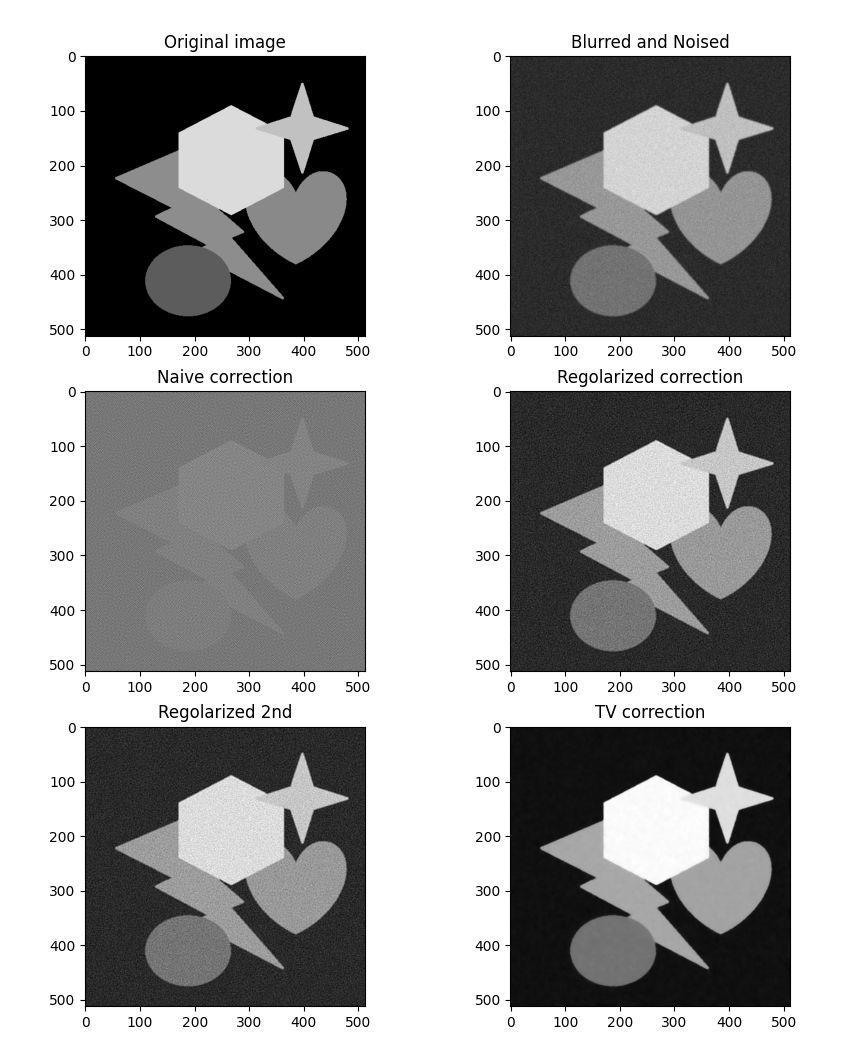
\includegraphics[width=14cm]{sample5}
    \caption{sample5.png - Dim. Kernel: $9\times9$, $\sigma:1.3$,Std. Dev.:$0.05$, $\lambda:0.08$}
    \end{figure}
    \newpage
    \begin{figure}[h!]
    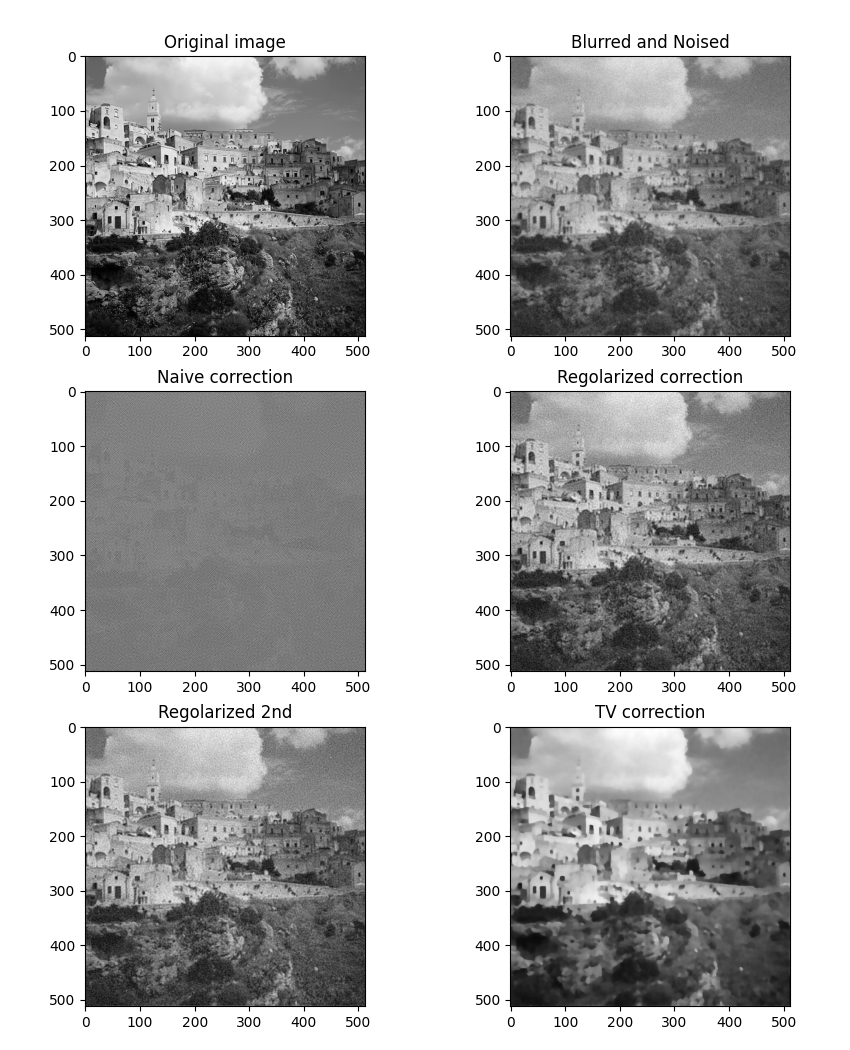
\includegraphics[width=14cm]{sample10}
    \caption{sample10.png - Dim. Kernel: $9\times9$, $\sigma:1.3$,Std. Dev.:$0.05$, $\lambda:0.08$}
    \end{figure}
    \newpage

\section{PSNR e MSE}
    L'analisi delle misure di PSNR e MSE va in contrasto con quanto osservato nelle immagini analizzate poc'anzi, in quando il valore di PSNR dell'algoritmo che implementa il metodo del gradiente con il parametro di regolarizzazione $TV$ è sempre superiore a quello degli altri algoritmi, nonostante come già riportato le immagini fotografiche risultino qualitativamente inferiori (almeno nel caso di un massimo di 100 iterazioni).
    
    Nel fare i test per raccogliere i dati sui valori di PSNR e MSE, abbiamo variato la dimensione del kernel, il valore di $\sigma$, la deviazione standard del rumore e il valore del parametro di regolarizzazione usando i valori indicati nella tabella \ref{table:1}. Di conseguenza abbiamo ottenuto 75 diversi valori del PSNR e del MSE per ogni algoritmo usato su una singola immagine, quindi 750 diversi valori per l'intero dataset. Dal momento che una tabella di simili dimensioni richiederebbe troppo spazio all'interno di questo documento, riportiamo in questa sede solo le tabelle con le medie dei valori ottenuti fra le 10 immagini di alcuni test scelti, mentre per i dati completi rimandiamo ai file .csv allegati.
    
    I parametri sono indicati, per motivi di spazio, con la notazione KX\_Y\_Z; dove X indica la dimensione e il valore di sigma del kernel (K1 equivale ad un kernel di dimensione $5\times5$ con valore di $\sigma=0.5$, K2 equivale ad una dimensione di $7\times7$ con $\sigma=1$ e K3 indica un kernel di dimensione $9\times9$ con $\sigma=1.3$), Y indica il valore della deviazione standard del rumore e Z il valore del parametro $\lambda$
    
    \begin{table}[!ht]
    \centering
    \begin{tabular}{|l|l|l|}
    \hline
        Parametri & Noised & Naive \\ \hline
        K1\_0.01\_0.01 & 32.88894160008047 & 20.906620556841617 \\ \hline
        K1\_0.02\_0.05 & 30.763199597344958 & 14.8915184413088 \\ \hline
        K1\_0.03\_0.08 & 28.663883887898002 & 11.362064451498266 \\ \hline
        K1\_0.04\_0.32 & 26.830940497683315 & 8.861122389375282 \\ \hline
        K1\_0.05\_1 & 25.248405184567638 & 6.925775031538379 \\ \hline
        K2\_0.01\_0.01 & 30.6251433086292 & 8.963663561306513 \\ \hline
        K2\_0.02\_0.05 & 29.216164594604077 & 2.8832589955413335 \\ \hline
        K2\_0.03\_0.08 & 27.61380043143138 & -0.6605537021630714 \\ \hline
        K2\_0.04\_0.32 & 26.084333732275887 & -3.1717769592303964 \\ \hline
        K2\_0.05\_1 & 24.697711613529346 & -5.12897412971146 \\ \hline
        K3\_0.01\_0.01 & 29.929334386094617 & 9.127820763357565 \\ \hline
        K3\_0.02\_0.05 & 28.696555087533152 & 3.0185527548672435 \\ \hline
        K3\_0.03\_0.08 & 27.238538348524095 & -0.5508328107608824 \\ \hline
        K3\_0.04\_1 & 25.81293328683397 & -3.06923303073812 \\ \hline
        K3\_0.05\_1 & 24.497025480815115 & -5.031814263063739 \\ \hline
    \end{tabular}
    \caption{PSNR medi in test scelti - 1 di 2}
    \label{table:2}
    \end{table}
    
    \begin{table}[!ht]
    \centering
    \begin{tabular}{|l|l|l|}
    \hline
        Tikhonov1 & Tikhonov2 & TV \\ \hline
        28.85365975216535 & 29.397966691454165 & 40.31057299355923 \\ \hline
        27.670014350466612 & 27.671699656368297 & 36.08971920069892 \\ \hline
        25.762903812128762 & 25.762935837422873 & 34.484105543977385 \\ \hline
        21.422057375046727 & 21.422037850812796 & 30.933612242387806 \\ \hline
        15.829495558542666 & 15.829497008321814 & 26.091522177092646 \\ \hline
        29.434919420524473 & 30.134660830205746 & 36.80653808537427 \\ \hline
        28.629106610405227 & 28.630959404346584 & 33.33733899438458 \\ \hline
        26.92191582698042 & 26.921951594230443 & 32.15791844794761 \\ \hline
        21.414643285159894 & 21.414641102545374 & 29.54942833094263 \\ \hline
        15.785529121228809 & 15.785529964147633 & 26.568120871033337 \\ \hline
        29.72394757943159 & 30.262901407284858 & 35.82801086265471 \\ \hline
        28.697946979382618 & 28.699329252764294 & 32.24991178120849 \\ \hline
        27.07183421922942 & 27.071855677963207 & 31.34081689896302 \\ \hline
        15.764980436419147 & 15.764980341189448 & 26.29792488491205 \\ \hline
        15.759412904341838 & 15.759412782636478 & 26.28418529950803 \\ \hline
    \end{tabular}
    \caption{PSNR medi in test scelti - 2 di 2}
    \label{table:3}
    \end{table}
    \newpage
    
    \begin{table}[!ht]
    \centering
    \begin{tabular}{|l|l|l|}
    \hline
        Parametri & Noised & Naive \\ \hline
        K1\_0.01\_0.01 & 0.0006202613738970486 & 0.008116005363064038 \\ \hline
        K1\_0.02\_0.05 & 0.0009200495559788917 & 0.03242379963657855 \\ \hline
        K1\_0.03\_0.08 & 0.0014203720800512248 & 0.07308063396449 \\ \hline
        K1\_0.04\_0.32 & 0.0021196805024182573 & 0.12998558476529137 \\ \hline
        K1\_0.05\_1 & 0.0030207608821427646 & 0.20296832304760967 \\ \hline
        K2\_0.01\_0.01 & 0.001085918247926105 & 0.12695419850205097 \\ \hline
        K2\_0.02\_0.05 & 0.0013847982893449005 & 0.5148542031796666 \\ \hline
        K2\_0.03\_0.08 & 0.0018846186466044122 & 1.1643121340880531 \\ \hline
        K2\_0.04\_0.32 & 0.002587434138046774 & 2.075795561872906 \\ \hline
        K2\_0.05\_1 & 0.0034893312156784517 & 3.2576827153152914 \\ \hline
        K3\_0.01\_0.01 & 0.0012855039280980532 & 0.12226438926550005 \\ \hline
        K3\_0.02\_0.05 & 0.001583168688714036 & 0.49907770364626425 \\ \hline
        K3\_0.03\_0.08 & 0.002083306295111171 & 1.135294215544004 \\ \hline
        K3\_0.04\_0.32 & 0.002786273571792625 & 2.0320524068670793 \\ \hline
        K3\_0.05\_1 & 0.0036816538874152203 & 3.185778647086994 \\ \hline
    \end{tabular}
    \caption{MSE medi in test scelti - 1 di 2}
    \label{table:4}
    \end{table}

    \begin{table}[!ht]
    \centering
    \begin{tabular}{|l|l|l|}
    \hline
        Tikhonov1 & Tikhonov2 & TV \\ \hline
        0.0013027055116812667 & 0.001149583071691836 & 0.00021320361464072734 \\ \hline
        0.0017322871994439597 & 0.0017316356193361894 & 0.000596598574595035 \\ \hline
        0.002707055930029478 & 0.0027070368482852614 & 0.0008063338394220963 \\ \hline
        0.008381850944323768 & 0.00838187641387138 & 0.001683702537001512 \\ \hline
        0.03137426721230338 & 0.03137425830704766 & 0.003528737461077555 \\ \hline
        0.0011694542274754201 & 0.0010089745799529877 & 0.0004911022352847949 \\ \hline
        0.0014825924673268407 & 0.0014820683691548443 & 0.0009266279516767339 \\ \hline
        0.0021959540590343247 & 0.00219593956665443 & 0.001131476087049577 \\ \hline
        0.008531570044950317 & 0.008531577767220527 & 0.00198253005385718 \\ \hline
        0.031699589253196526 & 0.03169958175532764 & 0.003343142680843672 \\ \hline
        0.0011341308420553908 & 0.0010229958160226937 & 0.0006145258161427157 \\ \hline
        0.001514555806438736 & 0.0015141971884928065 & 0.0010756762721259318 \\ \hline
        0.002184168807002595 & 0.002184160725997061 & 0.001274423882446191 \\ \hline
        0.008660220493829075 & 0.008660213155263583 & 0.0021114846846985317 \\ \hline
        0.03187803763787521 & 0.031878038702191525 & 0.003484314494466365 \\ \hline
    \end{tabular}
    \caption{MSE medi in test scelti - 2 di 2}
    \label{table:5}
    \end{table}
    \newpage

\section{Medie e Deviazioni standard}
    Abbiamo poi calcolato, per alcuni parametri fissati, i valori medi e la deviazione standard di PSNR e MSE calcolati sull'intero set di immagini, di seguito riportati.
    
    \subsection{PSNR - medie}
    
    \begin{table}[!ht]
    \centering
    \begin{tabular}{|l|l|l|}
    \hline
        Parametri & Noised & Naive \\ \hline
        K1\_0.02\_0.32 & 30.763768917410044 & 14.894662327258937 \\ \hline
        K1\_0.04\_0.08 & 26.828388450594588 & 8.878555041056844 \\ \hline
        K2\_0.01\_0.05 & 30.622021092621537 & 8.966179977846219 \\ \hline
        K2\_0.03\_0.01 & 27.6123416740849 & -0.6712866218224003 \\ \hline
        K2\_0.04\_1 & 26.078864556711757 & -3.1754732746047263 \\ \hline
        K3\_0.01\_0.32 & 29.93320745230278 & 9.123446234284177 \\ \hline
        K3\_0.03\_0.08 & 27.238538348524095 & -0.5508328107608824 \\ \hline
        K3\_0.05\_0.05 & 24.494076785889234 & -5.038541070382648 \\ \hline
    \end{tabular}
    \caption{PSNR medi - 1 di 2}
    \label{table:6}
    \end{table}
    
    \begin{table}[!ht]
    \centering
    \begin{tabular}{|l|l|l|}
    \hline
        Tikhonov1 & Tikhonov2 & TV \\ \hline
        21.7819230199858 & 21.781917748686006 & 31.04209033931886 \\ \hline
        23.92319272116348 & 23.923228522409865 & 34.110429553506364 \\ \hline
        30.55319797402757 & 30.553647157775565 & 33.51094774693016 \\ \hline
        21.223671230137814 & 22.298241259606492 & 34.238199848360786 \\ \hline
        15.79135726226173 & 15.791357125229187 & 26.581916894483562 \\ \hline
        21.522526143402864 & 21.52254410032735 & 29.281069470119412 \\ \hline
        27.07183421922942 & 27.071855677963207 & 31.34081689896302 \\ \hline
        24.107064541547256 & 24.11033325395355 & 31.8493174993012 \\ \hline
    \end{tabular}
    \caption{PSNR medi - 2 di 2}
    \label{table:7}
    \end{table}
    
    \subsection{PSNR - deviazioni standard}
    
    \begin{table}[!ht]
    \centering
    \begin{tabular}{|l|l|l|}
    \hline
        Parametri & Noised & Naive \\ \hline
        K1\_0.02\_0.32 & 1.658802250557476 & 0.023664854688653286 \\ \hline
        K1\_0.04\_0.08 & 0.8413523869964247 & 0.04102936694626389 \\ \hline
        K2\_0.01\_0.05 & 2.528216342828928 & 0.037568339882867924 \\ \hline
        K2\_0.03\_0.01 & 1.5775909212341903 & 0.01929727323852776 \\ \hline
        K2\_0.04\_1 & 1.228694278540623 & 0.03144829034933194 \\ \hline
        K3\_0.01\_0.32 & 2.572979136502637 & 0.0794215973211503 \\ \hline
        K3\_0.03\_0.08 & 1.697988459722755 & 0.046787544568358645 \\ \hline
        K3\_0.05\_0.05 & 1.0727261062834132 & 0.019264568863773632 \\ \hline
    \end{tabular}
    \caption{PSNR deviazioni standard - 1 di 2}
    \label{table:8}
    \end{table}
    
    \begin{table}[!ht]
    \centering
    \begin{tabular}{|l|l|l|}
    \hline
        Tikhonov1 & Tikhonov2 & TV \\ \hline
        2.6414685642821576 & 2.641456531489875 & 4.47106635598741 \\ \hline
        0.582326403868461 & 0.582333109259285 & 4.472359920936679 \\ \hline
        2.1722265542187214 & 2.17262796777723 & 4.3623408325974715 \\ \hline
        0.168900366912713 & 0.23339988763221314 & 3.687345818425936 \\ \hline
        2.7438990012612074 & 2.743898990910928 & 3.5386199772849665 \\ \hline
        2.637030803854423 & 2.6370477655094087 & 3.8724018388912054 \\ \hline
        1.8319794710385187 & 1.8319870258907323 & 3.788504784930772 \\ \hline
        0.8245022506762851 & 0.8251210295802458 & 3.8001097668308756 \\ \hline
    \end{tabular}
    \caption{PSNR deviazioni standard - 2 di 2}
    \label{table:9}
    \end{table}
    \newpage
    
    \subsection{MSE - medie}
    
    \begin{table}[!ht]
    \centering
    \begin{tabular}{|l|l|l|}
    \hline
        Parametri & Noised & Naive \\ \hline
        K1\_0.02\_0.32 & 0.0009206666823855502 & 0.03239964074415069 \\ \hline
        K1\_0.04\_0.08 & 0.0021212426730849833 & 0.12946843704967997 \\ \hline
        K2\_0.01\_0.05 & 0.0010866357436223138 & 0.12688146916889315 \\ \hline
        K2\_0.03\_0.01 & 0.0018846166708029646 & 1.1671668555503025 \\ \hline
        K2\_0.04\_1 & 0.002590376676267936 & 2.077584523963618 \\ \hline
        K3\_0.01\_0.32 & 0.00128372312619177 & 0.12238472318750179 \\ \hline
        K3\_0.03\_0.08 & 0.002083306295111171 & 1.135294215544004 \\ \hline
        K3\_0.05\_0.05 & 0.0036847659616542953 & 3.19049727608101 \\ \hline
    \end{tabular}
    \caption{MSE medi - 1 di 2}
    \label{table:10}
    \end{table}
    
    \begin{table}[!ht]
    \centering
    \begin{tabular}{|l|l|l|}
    \hline
        Tikhonov1 & Tikhonov2 & TV \\ \hline
        0.007900640217740363 & 0.007900639024825434 & 0.0016697098088447424 \\ \hline
        0.00409047235378353 & 0.004090439494530687 & 0.0008328573198533096 \\ \hline
        0.0010267168608407377 & 0.00102667258212427 & 0.0009119679331085184 \\ \hline
        0.007550422585664756 & 0.005899698857127317 & 0.0006414251034730055 \\ \hline
        0.03167385690244734 & 0.0316738579974414 & 0.0033387537952859593 \\ \hline
        0.00844051248572419 & 0.008440491067906617 & 0.002072074921199472 \\ \hline
        0.002184168807002595 & 0.002184160725997061 & 0.001274423882446191 \\ \hline
        0.003964789023405572 & 0.003961935515935415 & 0.001133074851968335 \\ \hline
    \end{tabular}
    \caption{MSE medi - 2 di 2}
    \label{table:11}
    \end{table}
    
    \subsection{MSE - deviazioni standard}
    \begin{table}[!ht]
    \centering
    \begin{tabular}{|l|l|l|}
    \hline
        Parametri & Noised & Naive \\ \hline
        K1\_0.02\_0.32 & 0.0005096930780202533 & 0.00017572064849211516 \\ \hline
        K1\_0.04\_0.08 & 0.0005114466053173154 & 0.0012258348994327946 \\ \hline
        K2\_0.01\_0.05 & 0.0009890410172708824 & 0.0010922683146856853 \\ \hline
        K2\_0.03\_0.01 & 0.0009832177594471577 & 0.005180408030698784 \\ \hline
        K2\_0.04\_1 & 0.00099050366592391 & 0.01502025453372986 \\ \hline
        K3\_0.01\_0.32 & 0.001187843289307018 & 0.0022018586655526227 \\ \hline
        K3\_0.03\_0.08 & 0.0011858666882446796 & 0.01218816494147507 \\ \hline
        K3\_0.05\_0.05 & 0.0011872505890449152 & 0.01414467738591752 \\ \hline
    \end{tabular}
    \caption{MSE deviazioni standard - 1 di 2}
    \label{table:12}
    \end{table}
    
    \begin{table}[!ht]
    \centering
    \begin{tabular}{|l|l|l|}
    \hline
        Tikhonov1 & Tikhonov2 & TV \\ \hline
        0.004603955767830908 & 0.004603938366165981 & 0.002745589109251268 \\ \hline
        0.0005905215539182448 & 0.0005905230761723575 & 0.0014339795159147126 \\ \hline
        0.0007187297309404321 & 0.0007188617410990995 & 0.001516779348411557 \\ \hline
        0.0003070971067675332 & 0.0003376151566664521 & 0.0009514944202030993 \\ \hline
        0.01850031934813074 & 0.018500320607146282 & 0.0038579942140794968 \\ \hline
        0.0052155250808946325 & 0.005215518899080878 & 0.0029939518379029344 \\ \hline
        0.0012360152796652784 & 0.0012360212772982882 & 0.001885354597321474 \\ \hline
        0.0009180381710769759 & 0.0009181889991335728 & 0.0016709918592897892 \\ \hline
    \end{tabular}
    \caption{MSE deviazioni standard - 2 di 2}
    \label{table:13}
    \end{table}
    
    \newpage

\section{}
    
    
\end{document}